\chap{Experimental Apparatus}
\label{chap:detector}
\section{The Large Hadron Collider}
\indent The Large Hadron Collider (LHC) is the world's most powerful particle accelerator. By accelerating protons to 99.9999991 percent of the speed of light and smashing them in head on collisions, the LHC hopes to probe some of the most fundamental questions of physics. The LHC sits in a circular tunnel 27 km in circumference under the Franco-Swiss border near Geneva, Switzerland. A diagram of the LHC complex is shown in figure \ref{LHC:fig:LHCComplex} ~\\
\begin{figure}[h!]
%\begin{center}
\centering
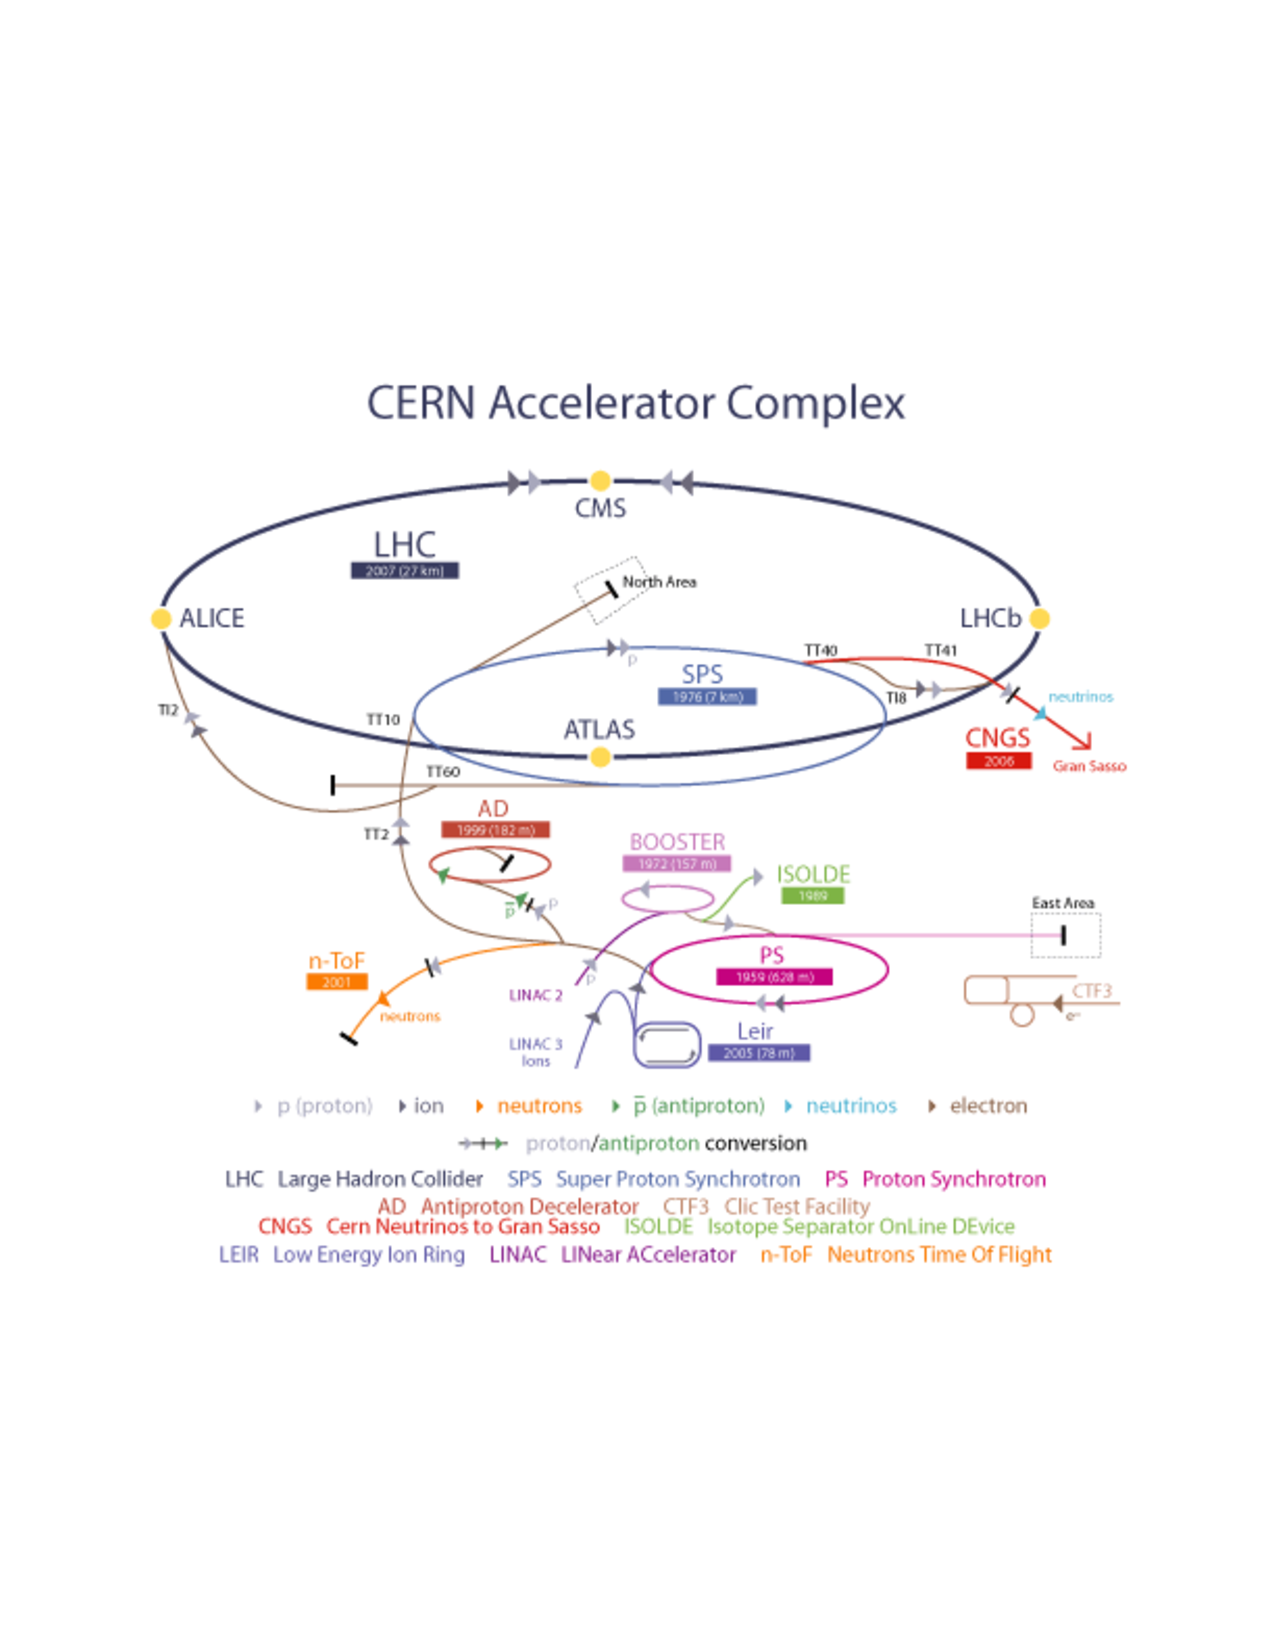
\includegraphics[width=0.85\textwidth, angle=270]{plots/AccComplex0700829.pdf}
\caption{ The Large Hadron Collider complex. (Taken from \cite{biblio:LHCpublic}) \label{LHC:fig:LHCComplex}}
%\end{center}
\end{figure}

\indent The LHC expands upon older particle accelerators. First protons are obtained by stripping electrons from hydrogen atoms. These protons are accelerated by LINAC2, a older linear accelerator at CERN, to 31.4 percent of the speed of light. The Proton Synchrotron Booster (PSB) then boosts the protons to 91.6 percent of the speed of light. These protons are then dumped into the Proton Synchrotron (PS) and accelerated to 99.93 percent of the speed of light. Afterwards, the protons enter the Super Proton Synchrotron (SPS). The SPS accelerate the proton to 99.9998 percent of the speed of light. At this point the energy of the proton is 450 GeV. These protons finally enter the LHC ring, which increases the proton energy to 3.5 TeV. This allows for a center of mass energy of 7 TeV during collisions. ~\\
\indent The LHC is designed to accelerate the protons to energies of 7 TeV, creating 14 TeV center of mass collisions. The LHC is scheduled to achieve this target energy in two years. ~\\
\indent The LHC has six particle detectors to detect the multitude of particles that are created during the collisions. The ALICE detector specializes in collisions of heavy ions. LHCb specializes in physics involving the bottom quark. TOTEM and LHCf are detectors measuring scattering cross sections, and diffractive processes, and cosmic ray physics. ATLAS and CMS are general purpose detectors optimized to detect a large spectrum of particles created by the proton proton collision. ~\\
\indent This analysis uses data collected by the ATLAS detector. ~\\
\section{The ATLAS Detector}
\label{LHC:detector}
\indent The ATLAS Detector is a general purpose detector that detects a multitude of particles that is created by the proton proton collisions. The detector is 25 meters high and 44 meters long and weights over 7000 tons.\cite{biblio:JINST} The detector consists of an inner tracking detector, the electromagnetic calorimeter, the hadronic calorimeter and the muon spectrometer. The structure of the ATLAS detector is shown in figure \ref{LHC:fig:ATLASDet} ~\\
\begin{figure}[h!]
%\begin{center}
\centering
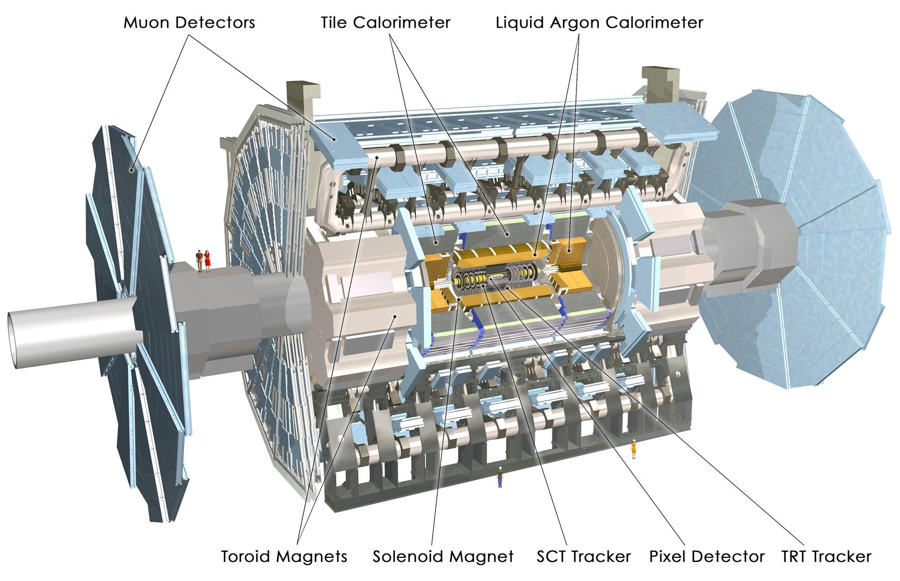
\includegraphics[width=0.75\textwidth, angle=0]{figures/ATLAS_detector_alles_mittel_EN.PNG}
\caption{ The ATLAS detector. Pixel, SCT, and TRT Detectors form the inner detector.  (Taken from \cite{biblio:JINST}) \label{LHC:fig:ATLASDet}}
%\end{center}
\end{figure}

\indent The inner tracker detector is located closest to the collision beam and tracks the path of charged particles such as electrons, and muons. The inner detector will be covered in further detail in section \ref{LHC:ID}. The electromagnetic calorimeter (EM calorimeter) surrounds the inner detector and measures the amount of energy of electromagnetic particles such as electrons and photons. The hadronic calorimeter surrounds the electromagnetic calorimeter and measures the amount of energy of hadrons such as protons and neutrons. The calorimeters are described in further detail in section \ref{LHC:Calorimeter}. The muon spectrometer forms the large outer layer of the detector, surrounding the hadronic calorimeter. Few particles other than muons and neutrinos can penetrate through the calorimeters. The muon spectrometer records the tracks left by the charged muons. The muon spectrometer is described in further detail in section \ref{LHC:MuonSpec}. Neutrinos are undetectable and must be inferred through conservation of momentum. A diagram of the signature left by each particle type is given in figure \ref{LHC:fig:ATLASParticleDiagram} ~\\
\begin{figure}[h!]
%\begin{center}
\centering
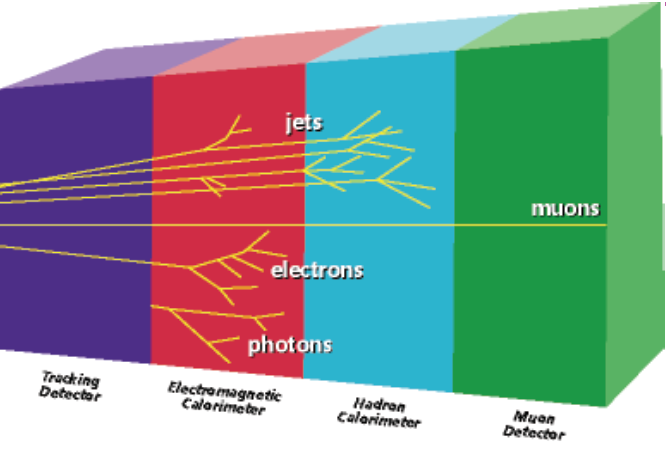
\includegraphics[width=0.55\textwidth, , angle=0]{figures/ATLAS_Particle_Diagram.PNG}
\caption{ The signature left by different particles. (Taken from \cite{biblio:SMcourse}) \label{LHC:fig:ATLASParticleDiagram}}
%\end{center}
\end{figure}

\indent A photon is not charged and so leaves no track. Photons do interact electromagnetically and therefore deposit all their energy in the EM calorimeter in the form of a cascading shower of electrons and photons. Electrons are charged and do leave a track in the inner detector and deposit their energy in the EM calorimeter. Pions and protons are charged and will leave a track in the inner detector, and they will deposit all their energy in the hadronic calorimeter. Neutrons are not charged and will not leave a track. Like protons, neutrons will deposit their energy in the hadronic calorimeter. Muons penetrate the detector and are charged. They will leave a track in both the inner detector and the muon spectrometer. ~\\
\indent Almost all particles that the ATLAS detector is looking for are unstable, meaning the particles will decay before they reach the detector. The final decay product is almost always a combination of the above particles and the undetectable neutrino. The original particle's kinematics is then calculated from the kinematics of each of its measurable decay products. ~\\
\indent Aproximately1000 particles are produced from the collision point every 75 nanoseconds at the Large Hadron Collider.\cite{biblio:JINST} The ATLAS Detector uses a system of triggers to filter this vast amount of data, recording only interesting collisions. The triggering system is complex and depends on the type of particle that is triggered on. This analysis uses the muon triggering system which is described in more detail in section \ref{LHC:MuonTrigger}. ~\\
\indent The ATLAS detector has two equivalent coordinate systems. The rectangular coordinate system x, y, z is defined as follows. The z direction points in the direction of the beam pipe. The positive x direction points to the center of the LHC ring. The positive y direction points in the upward direction. The origin is defined as the center of the ATLAS detector and lie on the center line of the beam pipe. Alternatively, Radius R is defined as the distance from the z axis (also the beam axis). The azimuthal angle $\phi$ is measured around the beam axis, and the polar angle $\theta$ is the angle from the beam axis. Frequently, the pseudorapidity, defined as $\eta =$ - ln~tan$({\theta}/2)$, is used in place of $\theta$ as the third coordinate. ~\\
\subsection{The Inner Detector}
\label{LHC:ID}
\indent The inner detector surrounds the collider beam tube and tracks the path of charged particles including electrons, charged pions, protons, and muons. Figure \ref{LHC:fig:ATLASID} shows the configuration of the inner detector. ~\\
\begin{figure}[h!]
%\begin{center}
\centering
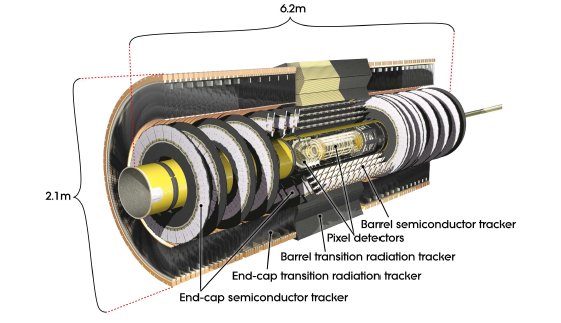
\includegraphics[width=0.75\textwidth, angle=0]{figures/ATLAS_ID_Detector.PNG}
\caption{ Cutaway view of the ATLAS inner detector.  (Taken from \cite{biblio:JINST}) \label{LHC:fig:ATLASID}}
%\end{center}
\end{figure}

\indent The inner detector consists of two silicon semiconductor detectors; the Pixel detector and the Semiconductor Tracker (SCT) and a straw tracker called the Transition Radiation Tracker (TRT). The three detectors operate independently of one another but the information they gather is combined during reconstruction to form a complete track of the particle as it flies through the inner detector. The whole inner detector is immersed in a 2 T magnetic field produced by a solenoidal superconducting magnet that radially surrounds the whole inner detector. At this radii, around 1000 particles will emerge from the collision point every 75 ns demanding that the inner detector have good position and time resolution. \cite{biblio:JINST} ~\\ 
\indent The Pixel detector lies closest to the beam pipe. The Pixel detector uses thousands of pixels of doped silicon that form diodes. The diodes are placed in reverse bias within the larger electronic circuit. Hence no current will flow through the circuit unless the diode breaks down. As a charged particle pass through the diode, they cause small ionizations that momentarily breaks down the diode, allowing current to flow. This current can then be detected and measured. ~\\
\indent The Pixel detector has three layers of pixel sensors in the cylindrical barrel and three wheels of pixel sensors in the endcaps covers a total $|\eta|$ of 2.5. The pixels measures both the $\phi$ and Z coordinate of the hit simultaneously, achieving 10 ${\mu}m$ accuracy in the (R - $\phi$) direction and 115 ${\mu}m$ in the Z direction in the barrel and 10 ${\mu}m$ resolution in the (R - $\phi$) direction and 115 ${\mu}m$ in the R direction in the endcap. \cite{biblio:JINST} ~\\
\indent At larger radii, the SCT surrounds the Pixel detector. The SCT operates in a similar fashion to the Pixel detector as the SCT is also a silicon detector. Instead of pixels of doped silicon, the SCT uses narrow strips of doped silicon. Narrow strips allow measurement of only one coordinate (either the $\phi$ or Z and not both like the Pixel Detectors) per strip but is more cost effective. To compensate for this, the SCT use two orthogonally oriented strips glued back to back to measure both coordinates. The SCT has four planes of these double strips in the cylindrical barrel and four wheels in the endcaps. The SCT can achieve position accuracies of 17 ${\mu}m$ in the (R-$\phi$) direction and 580 ${\mu}m$ in the Z direction in the barrel and 17 ${\mu}m$ in the (R-$\phi$) direction and 580 ${\mu}m$ in the R direction in the endcap. \cite{biblio:JINST} ~\\
\indent The TRT lies at a larger radii around both the SCT and the Pixel detector and covers an |$\eta$| range of 2.0. Unlike the two silicon detectors, the TRT is a straw tracker and is filled with around 300 thousand wire straws. The straws is filled with a combination of xenon, $CO_2$, and $O_2$ gas. As a charged particle flies through the straw, it ionizes that gas within the straw. Voltage is applied to the wall of the straw and the central wire making the straw a capacitor. The positive gas ions and negative free electrons will follow the electric field lines of the capacitor and drift in opposite directions to the central wire and straw wall. The speed of the electron drift is known and based on the timing of the arrival of the first election and the last election, the distance from the center of the straw to the flight path of the charged particle can be determined. This allows the measurement of one coordinate of the particle's flight. This process is shown in figure \ref{LHC:fig:StrawTube}. \cite{biblio:JINST} ~\\
\begin{figure}[h!]
%\begin{center}
\centering
%\includegraphics[width=0.5\textwidth]{plots/ATLAS_Staw_Tube_Fig.pdf}
\includegraphics[width=0.3\textwidth]{figures/ATLAS_Staw_Tube_Fig.PNG}
\\
\caption{ Cross-section of a straw tube with an interacting muon. (Taken from\cite{biblio:JINST}) \label{LHC:fig:StrawTube}}
%\end{center}
\end{figure}

\indent The TRT's straws in the barrel and endcaps are arranged to measure the $\phi$ coordinate of the passing charged particle. The $\phi$ direction is the direction in which charged particles bend. Therefore, the TRT helps to measure the momentum of the charged particle. The TRT provides (R-$\phi$) direction information with an intrinsic accuracy of 130 mm per straw. This large resolution uncertainty is compensated by the large number of hits which a particle leaves in the TRT (around 36 hits per track is expected compared to 8 in the SCT and 3 in the Pixel). ~\\
\indent The TRT also aids in electron identification. The space between the straws is filled with materials with different indexes of refraction. When ultra-relativistic charged particles crosses the boundaries of different materials, they produce transition radiation. The transition radiation will in turn further ionize the gas in the straw, producing a high threshold hit in the straw. Particles with small invariant masses such as electrons are more likely to emit transition radiation. This allows for another form of electron identification and complements the electron identification function of the calorimeter. ~\\
\indent The hits in all three detectors are reconstructed into a track of the flight path of the charged particle by ATLAS reconstruction software. Depending on the curvature of the track, the momentum and charge of the particle can be measured. By matching the track to other signals in the calorimeter or the muon spectrometer, the identity of the charged particle can be determined. ~\\
\subsection{The Calorimeter}
\label{LHC:Calorimeter}
\indent The calorimeter is separated into two types. The electromagnetic calorimeter (EM calorimeter) is designed to measure the energy of electromagnetic particles such as electrons and photons, and the hadronic calorimeter is designed to measure the energy of hadrons such as protons, neutrons, and pions. The calorimeter covers up to an $\eta$ range of $|\eta| < 4.9$. The calorimeter is not only used to measure the energy of jets and particles but also used to reduce the probability of a non-muon particle from punching through to the outer muon detectors. Therefore the total thickness of the EM calorimeter is greater than 22 radiation lengths ($X_0$) in the barrel and greater than 24 $X_0$ in the end-caps.\cite{biblio:JINST} The cut away view of the whole calorimeter is show in figure \ref{LHC:fig:ATLASCalo} ~\\
\begin{figure}[h!]
%\begin{center}
\centering
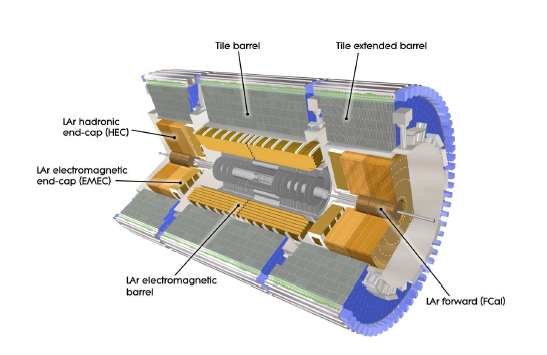
\includegraphics[width=0.75\textwidth, angle=0]{figures/ATLAS_Calo.PNG}
\caption{ The ATLAS calorimeter. (Taken from \cite{biblio:JINST}) \label{LHC:fig:ATLASCalo}}
%\end{center}
\end{figure}

\indent The inner most calorimeter is the liquid argon electromagnetic calorimeter (EM Calorimeter). The EM calorimeters are made of multiple planes of 1.5 mm thick lead plates. The 4 mm gap between the lead plates is filled with liquid argon. When high energy electrons or photons hit the lead plates they produce more electron-positron pairs through pair production. These newly produced electrons and positrons then will also produce more photons as they fly through the lead plates. This results in a shower of electrons and positrons until the photons no longer have enough energy to pair-produce. When the charged particles traverse the liquid argon, they ionize the argon. These ions and free electrons in the liquid argon drift to external electric terminals and are sensed as a current. The more energetic the initial electron or photon, the more electron - positron pairs will be produced causing a greater ionization in the liquid argon. Also, the more energetic the initial electron or photon, the deeper the electron shower will penetrate the calorimeter before it runs out of energy to produce more electron - positron pairs. Both are used to measure the total energy of the initial electromagnetic particle. The barrel part of the electromagnetic calorimeter covers up to an $|\eta| < 1.475$ and the two endcaps covers the $\eta$ range of $1.375 < |\eta| < 3.2$. ~\\
\indent Outside the electromagnetic calorimeter lie the hadronic calorimeter. The hadronic calorimeter is formed by three different detectors, the barrel tile calorimeter, the hadronic endcap calorimeter (HEC) and the forward hadron calorimeter (FCal). The barrel tile calorimeter covers an $\eta$ range $|\eta| < 1.0$ and two extended barrel tile calorimeter covers $0.8 < |\eta| < 1.7$. The tile calorimeter consists of multiple steel plates with scintillating tiles sandwiched in between. When hadrons such as protons, neutrons, pions, and kaons pass, they interact with the nuclei in the steel via the strong force and produce more hadrons. Those hadrons in turn interact with more steel nuclei eventually producing a shower of hadronic particles. As the hadrons pass the scintillating tiles, they cause the tiles to produce light that is amplified by a photomultiplier tube and then detected. The more energetic the initial hadron, the more hadrons produced in the hadronic shower and the more light is produced in the tiles. Also the more energetic the initial hadron, the deeper the hadronic shower penetrates before the hadrons no longer have enough energy to produce more hadrons. The HEC and the FCAL extends the $\eta$ coverage of the hadronic calorimeter to an |$\eta$| of 4.9. Both are liquid argon calorimeters and operate in the same way as the EM calorimeter. The HEC uses copper instead of lead plates because copper is better at interacting with hadrons than lead. For the same reason, the FCAL uses copper-tungsten plates in place of lead.~\\
\subsection{The Muon Spectrometer}
\label{LHC:MuonSpec}
\indent The muon spectrometer tracks muons with high enough energy to penetrate the calorimeter. Few particles other than muons and the undetectable neutrino can penetrate the large calorimeter. The muon spectrometer consist of two precision tracking detectors, the Monitored Drift Tube (MDT) and the Cathode Strip Chamber (CSC), and two detectors used in muon triggering, the Resistative Plate Chambers (RPC) and the Thin Gap Chambers (TGC). The muon triggering system is discussed in more detail in \ref{LHC:MuonTrigger}. The configuration of the muon system is shown in figure \ref{LHC:fig:ATLASMuonSpec} ~\\
\begin{figure}[h!]
%\begin{center}
\centering
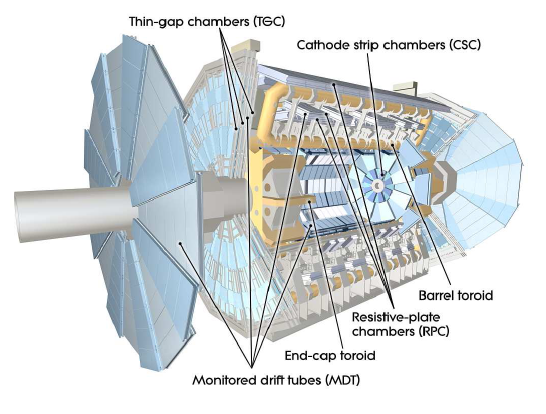
\includegraphics[width=0.75\textwidth, angle=0]{figures/ATLAS_MuonSpec.PNG}
\caption{ Cutaway view of the ATLAS Muon Spectrometer. (Taken from \cite{biblio:JINST}) \label{LHC:fig:ATLASMuonSpec}}
%\end{center}
\end{figure}

\indent The muon spectrometer is immersed in a magnetic field produced by eight superconducting toroid magnets in the barrel and eight superconducting toroid magnets in the endcaps. The barrel magnets cover an |$\eta$| range of 1.4 and the endcap magnets cover an |$\eta$| range from 1.6 to 2.7. The area with $1.4 < |\eta| < 1.6$ is called the transition region with a mixed magnetic field from both the barrel and endcap. The endcap magnets are offset from the barrel magnets by 22.5 degrees in the $\phi$ direction to allow a smoother magnetic field in this region. The configuration of the magnets is shown in figure \ref{LHC:fig:ATLASMag} ~\\
\begin{figure}[h!]
%\begin{center}
\centering
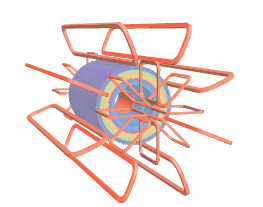
\includegraphics[width=0.60\textwidth, angle=270]{figures/ATLAS_ToroidMag.PNG}
\caption{ Geometry of the barrel and endcap toroid magnets. The cylinder repesents the calorimeter. (Taken from \cite{biblio:JINST}) \label{LHC:fig:ATLASMag}}
%\end{center}
\end{figure}

\indent The magnetic field bends the charged muons in the $\eta$ direction. The bending power of the magnets depends on the direction of muon travel. In the pseudorapidity range $0 < |\eta|< 1.4$, the barrel toroid provides 1.5 to 5.5 Tm of bending power. In between $1.6 < |\eta| < 2.7$, the end-cap toroids provide approximately 1 to 7.5 Tm of bending power. The bending power is lower in the transition region. ~\\
\indent The path of the muon can be reconstructed and the momentum of the muon can be measured from the amount of bending. The size of the muon spectrometer combined with the inner detector allows ATLAS to track muons over long distances. This is important because longer tracks mean more precise momentum measurements.\cite{biblio:JINST} ~\\
\indent The Monitored Drift Tube (MDT) consists of three to eight layers of drift tubes and covers an $\eta$ range of |$\eta$| < 2.7. The inner-most layer of the MDT only covers up to an $\eta$ range of |$\eta$| < 2.0. In the $\eta$ range between $2.0 < |\eta| < 2.7$, the Cathode Strip Chamber (CSC) replaces the MDT inner layer. ~\\
\indent The drift tubes of the MDT functions in the same manner as the straw tubes of the TRT in the inner detector. The muon ionizes the gas inside the tube and frees electrons. These electrons drift to the central wire of the drift tube because of the voltage difference between the central wire and the tube wall. The arrival of the electrons creates a pulse of current that is registered as a hit. How drift tubes operate is discussed in more detail in section \ref{LHC:ID}. The purpose of the MDT is to precisely measure the coordinates of the muon flight path in the bending $\eta$ direction. This measurement of the bending coordinate is used in the calculation of the momentum of the muon. The resolution of the MDT is 80 $\mu$m per tube.\cite{biblio:JINST}~\\
\indent The CSC replaces the inner MDT layer in the forward $\eta$ ranges between 2.0 and 2.7. This is needed because in this section the expected density of muons exceeds the safe operational limits of the MDT.\cite{biblio:JINST} The CSC is formed with multiwire proportional chambers. The chambers are formed with strips of cathode capacitor plates on either side and a row of anode wires sandwiched in between. As a charged particle flies through the chamber it will ionize the gas in the chamber, freeing electrons and positively charged ions. The free electron will drift along electric field lines to the nearest wire and the ions will drift to the cathode plates strips. Different electrons may end up in different wires as the ionization area has some spread and different ions on different strips. The CSC then regresses the position of the muon from the proportions of signal in each strip. The structure of the CSC is show in figure \ref{LHC:fig:ATLASCSC}. ~\\
\begin{figure}[h!]
%\begin{center}
\centering
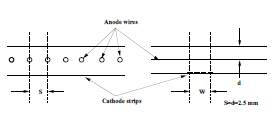
\includegraphics[width=0.50\textwidth, angle=0]{figures/ATLAS_CSC.PNG}
\caption{ Diagram of a plane in the ATLAS Cathode Strip Chamber. (Taken from \cite{biblio:JINST}) \label{LHC:fig:ATLASCSC}}
%\end{center}
\end{figure}

\indent The wires are arranged in the radial direction. This allows the wires to measure the $\phi$ coordinate of the muon. On one side, the cathode strips are arranged parallel to the wire to complement the measured $\phi$ coordinate of the muon and to reduce noise levels. On the other side, the cathode strips are arranged transverse to the wires to measure the $\eta$ coordinate of the muon. The resolution achieved by the CSC is 40 $\mu$m in the bending $\eta$ plane and about 5mm in the transverse$\phi$ plane. The difference is because the $\eta$ coordinate is measured by the cathode strips and the $\phi$ coordinate is measured by the wires. \cite{biblio:JINST} ~\\
\indent The RPC and TGC are trigger chambers with the goal of quickly measuring the position of the muon. The RPC chamber is formed by two orthogonal planes of cathode and anode strips. The gas in between the planes is chosen such that the gas sparks when a muon passes through. The sparking allow near-instantaneous detection of muons instead of waiting for the electrons and ions to drift onto the plates. The two orthogonal planes measure both the $\eta$ and $\phi$ coordinates of the muon track. The RPC extends out to an $|\eta|$ of 1.05 and covers the barrel of the detector. The TGC is a multiwire proportional chambers and operates similarly to the CSC. The TGC covers the $|\eta|$ range between 1.05 and 2.7 and covers the endcaps of the detector. However, the TGC can only trigger up to an $|\eta|$ of 2.4. The trigger system and software is described in section \ref{LHC:MuonTrigger}. ~\\
\indent The MDT can only measure the $\eta$ coordinate and not the $\phi$ coordinate of the muon. To compensate for this, the MDT chamber hits are matched to the respective RPC or TGC chamber hits and uses the $\phi$ coordinate of the trigger chamber as the second coordinate of the hit. If more than one muon passes through an MDT and trigger chamber pair then there is no unambiguous method to match the hits. Therefore the muon density in the MDT chambers must be low. Fortunately, simulations show that the number of muons that reach the muon spectrometer with $P_T > 6$ GeV is about $6*10^{-3}$ per beam-crossing, corresponding to about $1.5*10^{-5}$ per chamber.\cite{biblio:JINST} Assuming uncorrelated tracks, the probability of finding more than one track in any MDT/trigger chamber pair is very small. \cite{biblio:JINST} If two muons do traverse the same chamber, then the corresponding inner detector tracks of the muons are used to resolve the ambiguity. ~\\
\indent The hits recorded by the muon spectrometer detectors are reconstructed into the track of the flight path of the muon. The muon track is then matched to the inner detector track of the muon by the ATLAS reconstruction software MuID and STACO. This forms one complete combined muon track that traverses the whole ATLAS detector. The uncertainty of the momentum measurement is inversely related with the length of the track. Therefore, the long length the combined muon track serves to give precise measurements of the momentum of the muon. ~\\
\subsection{The Muon Trigger System}
\label{LHC:MuonTrigger}
\indent The ATLAS triggering system consists of three levels of triggers. At each level, more information is acquired for the event and the trigger refines the decision on whether the event is interesting. Because interesting events corresponds to high energy particles, the muon trigger selects high transverse momentum ($P_T$) muons. The first level trigger (L1 trigger) makes a decision in less than 2.5 ${\mu}s$ and reduces the rate of data collection to 75 kHz.\cite{biblio:JINST} The two higher level triggers, the Level 2 trigger (L2 trigger) and the event filter, further reduces the data recording rate to 200 Hz. \cite{biblio:JINST} ~\\
\indent For muons, the ATLAS L1 trigger depends on information gathered by the Resistive Plate Chambers (RPC) and the Thin Gap Chambers (TGC) detectors to quickly estimate the muon's $P_T$. ~\\
\indent The L1 RPC trigger compares the hit pattern of the measured muon to the theoretical infinite momentum muon to estimate the $P_T$ of the muon. The trigger electronics draws a line from the collision point to the hit in the middle 'pivot' layer of the RPC. If the muon has high transverse momentum we would expect a hit in both the inner and outer layer of the detector that are close to being on a straight line from the origin. If the transverse momentum of the muon is low then we would expect a hit that is far from a straight line in the inner layer and either a far away hit or no hit in the outer layer. The distance of the hits from the theoretical straight line is used to quickly estimate the $P_T$ of the muon without reconstructing the track of the muon. For the TGC detector, the pivot layer is the outer layer due to the positioning of the endcap magnets. This process is show schematically in figure \ref{LHC:fig:RPCTriggerAlg}. ~\\
\begin{figure}[h!]
%\begin{center}
\centering
\includegraphics[width=0.70\textwidth, angle=0]{figures/l1_algo.PNG}
\caption{ The Level 1 Trigger Algorithm used to estimate the $P_T$ of muons using the RPC and TGC Detector. (Taken from \cite{biblio:TriggerTwiki}) \label{LHC:fig:RPCTriggerAlg}}
%\end{center}
\end{figure}

\indent The L2 algorithm reconstructs the tracks of the muons which pass the L1 Trigger and get a more precise measurement of the muon $P_T$. With this information, the L2 trigger refines the decision on whether to keep the event. The rate of events which pass the L2 trigger is reduced to around 2 kHz. If the event passes the L2 trigger, the event filter (EF) reconstructs combined muons, calorimeter measurements, and vertices with more precise software. The EF software reduces the rate of events that will be fully reconstructed offline to a manageable 200 Hz. The trigger system is summarized in figure \ref{LHC:fig:MuonTrigFlow}. ~\\
\begin{figure}[h!]
%\begin{center}
\centering
\includegraphics[width=0.70\textwidth, angle=270]{plots/SchemaMuonTriggerSlice.pdf}
\caption{ Flow chart of the muon trigger system. (Taken from \cite{biblio:TriggerTwiki}) \label{LHC:fig:MuonTrigFlow}}
%\end{center}
\end{figure}

